\chapter{Theory}

Before describing the work on friction estimates that has been done, it is important to have some knowledge within vehicle dynamics, including basic knowledge on how tires and also different differentials work. The following chapter tries to describe this so that the reader has the right basic knowledge needed.

\section{Vehicle dynamics}

\subsection{Normal forces}


\subsection{The bicycle model}
The bicycle model is often used as a simplified way of describing vehicle dynamics.

\begin{figure}[h]
	\centering
	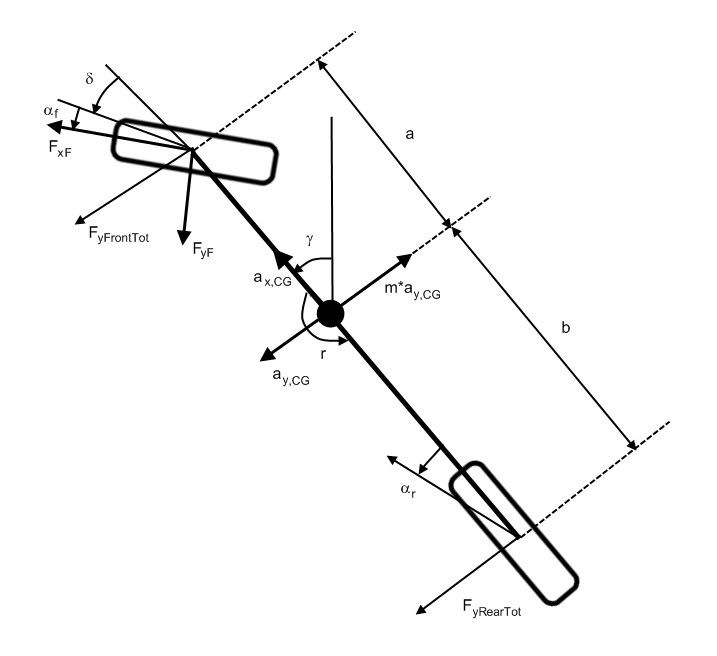
\includegraphics[width=0.8\textwidth]{Pictures/bicycle_model}
	\caption {Bicycle Model. \cite{fordonsdynamik99}}
	\label{bicycle_model}
\end{figure}

\section{Tire dynamics}

A tire that is non loaded will have a radius called unloaded radius. When a tire is loaded, and therefore have a normal force acting from the ground, it will deform against the contact area to the ground. This deformation will lead to a shorter radius to the ground, called the effective rolling radius. 

\subsection{Longitudinal forces}

Without torque acting on the tire, there will be rolling resistance due to higher compressing in the tire/road compression area then in the expansion area.
\begin{equation}
RollingResistance = \frac{F_{resistance}}{F_{z}}
\end{equation}
When a longitudinal force is acting on the tire, traction or braking, the tire will have more compression/expansion and a slip will occur. The longitudinal slip, $ \kappa $ is defined as
\begin{equation}
\kappa = \dfrac{R_{e}\omega-V_{x}}{V_{x}}
\end{equation}
Where $V_{x}$ is the nominal velocity, $R_{e}$ the effective rolling radius, and $\omega$ the angular velocity of the wheel. This leads to the following slip with different angular velocities:
\begin{equation}
Braking: \omega = 0 \Rightarrow \kappa = -1
\end{equation}
\begin{equation}
Free rolling: \omega = \frac{V}{R_{e}} \Rightarrow \kappa = 0
\end{equation}
\begin{equation}
Spinning: \omega = 2\frac{V}{R_{e}} \Rightarrow \kappa = 1
\end{equation}
The longitudinal force that will be acquired depends on the normal force, $ F_{z} $ and the friction used, $ \mu(s) $.
\begin{equation}
F_{x} = F_{z}\mu(s)
\end{equation}
The used friction will increase with the slip ratio until the maximum friction is met. This is when full gliding occurs. 

\subsection{Lateral forces}

Cornering stiffness
\begin{equation}
C_{y} = \frac{\delta F_{y}}{\delta}
\end{equation}
Where $\delta$ is the steering wheel angle.

Self aligning torque
\begin{equation}
M_{z} = F_{y}t_{p}
\end{equation}
Where $ F_{y} $  is the lateral force acting on the tire and $ t_{p} $ its distance to the center of the wheel. 

The lateral force acting on the wheel depends on its slip angle
\begin{equation}
F_{y}=C_{F}\alpha
\end{equation}
This can only be used in the linear part of the tire force/slip angle relationship. 



\section{Tire models}

There are several models to describe a tire mathematically. These models can be divided into four categories, empirical models, models using the similarity method, simple physical models and complex physical  models. 

Empirical models describe tire characteristics that are acquired from measurements of the tire. To fit the curve according to measured data the parameters are assessed with methods like regression. A well-known empirical model is the Magic Formula \cite{pacejka}. This model provides good fit for $F_{x}$, $F_{y}$ and $M_{z}$ curves and have coefficients that's easy to interpret.

Models using the similarity method are semi-empirical which means that some calculations are replaced by known or measured data. By distorting, rescaling and multiplying the result new relationships are acquired which can describe the tire in different situations. For example one can observe that that the pure slip curves shape doesn't change much \cite{pacejka} when the tire runs on different conditions. By shifting the nominal curve these conditions can be described.

The physical models are purely analytical and aims to describe the tire with help of its physical characteristics. A simple physical model uses simple mechanical representation and can be calculated fairly easy by hand. This often results in pretty poor accuracy but sometimes that's enough. To get better accuracy a more complex model can be set up and simulated in a computer using aids like the finite element method. 

\begin{figure}[h]
	\centering
	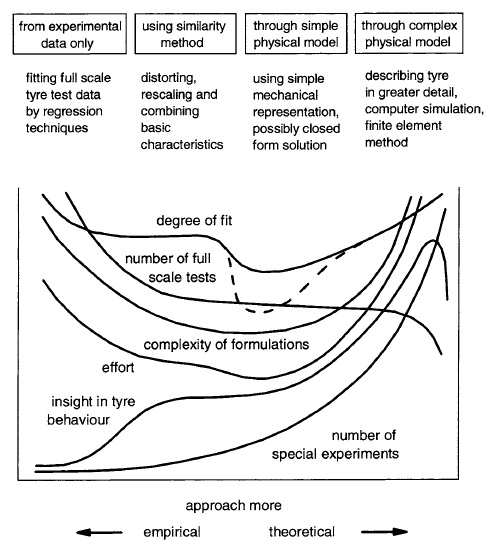
\includegraphics[width=0.8\textwidth]{Pictures/tire_modeling}
	\caption{Four categories of possible types of approach to develop a tire model. \cite{pacejka}}
	\label{tire_modeling}
\end{figure}

In Figure \ref{tire_modeling} some modeling characteristics and how they behave depending on category can be seen.

\subsection{Brush model}


\section{Differentials}


\subsection{Open differential}

With an open differential, the torque will be evenly distributed on the two wheels, but the velocities can be different. This means that the inner wheel will have a lower velocity in a corner, due tu its smaller turning radius. When one wheel has significant lower resistant then the other, its velocity will become much higher due to the same amount of torque. Two possible scenarios for this is when you climb a hill with different friction on the two tires and when you take corner fast leading to the inner wheel lifting from the ground. Both of these scenarios will lead to very high speeds on the wheel on the low $ \mu $ surface respectively the inner lifting wheel. The torque that the non-spinning wheel can transfer to the ground will be the same amount that the spinning wheel can transfer, leading to significant lower traction than what actually is available on the wheels.

A solution in these different scenarios would be to lock the differential. This would lead to that the two wheels would have the exact same velocity, and therefore not the same torque in certain situations. 

Side-gear and crown wheel angular velocities:
\begin{equation}
	-1 = \frac{\omega_{1} - \omega_{r}}{\omega_{2} - \omega_{r}}
\end{equation}
\begin{equation}
	\omega_{r} = \frac{\omega_{1} + \omega_{2}}{2}
\end{equation}



\subsection{Limited slip differential}

The goal with a limited slip differential (LSD) is to not apply more torque to a wheel then it can transfer to the ground.

\subsection{FXD}

Does not create under steering like locking torque LSD's. 

Lightweight alternative  to improve traction performance. Very little extra fuel consumption. Pre-emptive lock torque for take off. Wheel slip control. Yaw damping. 

If ABS or ESP is active, the FXD function is shutout. 

"Side pull reduction"


\subsubsection{Control algorithm}

Signals available for the control algorithm through CAN:
\begin{itemize}
	\item 4x Wheel speeds
	\item Engine torque
	\item Engine speed
	\item Accelerator position
	\item Brake Pedal Active
	\item ABS active
	\item ESP torque request, opening request (slow/fast)
	\item Yaw rate
	\item Steering wheel angle
	\item Lateral acceleration
\end{itemize}

Other signals that are used are estimated:

Vehicle speed.
Tire size difference.
Tire stiffness???
Lateral acceleration???



\subsubsection{Applying pressure}

By applying higher current to the pump, it will spin faster and thus creating larger centrifugal forces. This force will block the oil from exiting the pump, leading to a higher pressure within the pump. This pressure is also applied to the clutch which will press the clutch discs together and locking the axles together.

\subsection{How differentials affect vehicle handling} 

\section{Tire/road friction models/methods}

There have been extensive research within this field for the last fifty years and this results in many different approaches to model tire/road friction. Some of the more relevant models/methods for this work will be presented here.

\subsection{Mue}

\subsection{Slip-based friction model}
